%% V1.0
%% by Gabriel Garcia, gabrcg@gmail.com
%% This is a template for Udacity projects using IEEEtran.cls

%% Be Udacious!

\documentclass[10pt,journal,compsoc]{IEEEtran}

\usepackage[pdftex]{graphicx}    
\usepackage{cite}
\usepackage{hyperref}
\hyphenation{op-tical net-works semi-conduc-tor}


\begin{document}

\title{Map My World}

\author{Ghee Chong Foo}

\markboth{Map My World project, Robotics Nanodegree Program, Udacity}%
{}
\IEEEtitleabstractindextext{%

\begin{abstract}

In this write up, Simultaneous Localization and Mapping (SLAM) technique is used to perform mapping.  In particular, the Real Time Appearance Based Mapping (RTAB-Map) which utilizes Graph-SLAM algorithm.  A Udacity provided kitchen environment was mapped, followed by a custom environment.  In both cases a robot equipped with depth camera was driven around manually to perform mapping with at least 3 loop closures on the rtabmap database.

\end{abstract}

% Note that keywords are not normally used for peerreview papers.
\begin{IEEEkeywords}
Robotics, SLAM, RTAB-MAP.
\end{IEEEkeywords}}


\maketitle
\IEEEdisplaynontitleabstractindextext
\IEEEpeerreviewmaketitle
\section{Introduction}
\label{sec:introduction}

\IEEEPARstart
{S}imultaneous localization and mapping (SLAM) is a technique in robotics to construct and update a map of an unknown environment while at the same time keeping track of whereabout of the robots \cite{SLAM}.  This appears to be a chicken-and-egg problem and resolved through approximation using method such as particle filter, extended Kalman filter and Graph-SLAM.  In this project RTAB-Map (Real-Time Appearance-Based Mapping) that utilizes RGB-D Graph-SLAM approached will be deployed, which is based on global Bayesian loop closure detector.  The loop closure detector uses bag-of-words approach to determine the likelihood of new image comes from a previous location or a new location \cite{RTAB-MAP}

%{T}{he} introduction should provide some material regarding the history of the problem, why it is important and what is intended to be achieved. If there exists any previous attempts to solve this problem, this is a great place to note these while conveying the differences in your approach (if any). The intent is to provide enough information for the reader to understand why this problem is interesting and setting up the conversation for the solution you have provided
%Use this space to introduce your localization task and how you wish to accomplish it; save the details about the robot construction for later (simulation is a good point for this information). 
%If you have any papers / sites / repositories you have referenced for your robot, please make sure to cite them.

%example for inserting image
\begin{figure}[thpb]
      \centering
      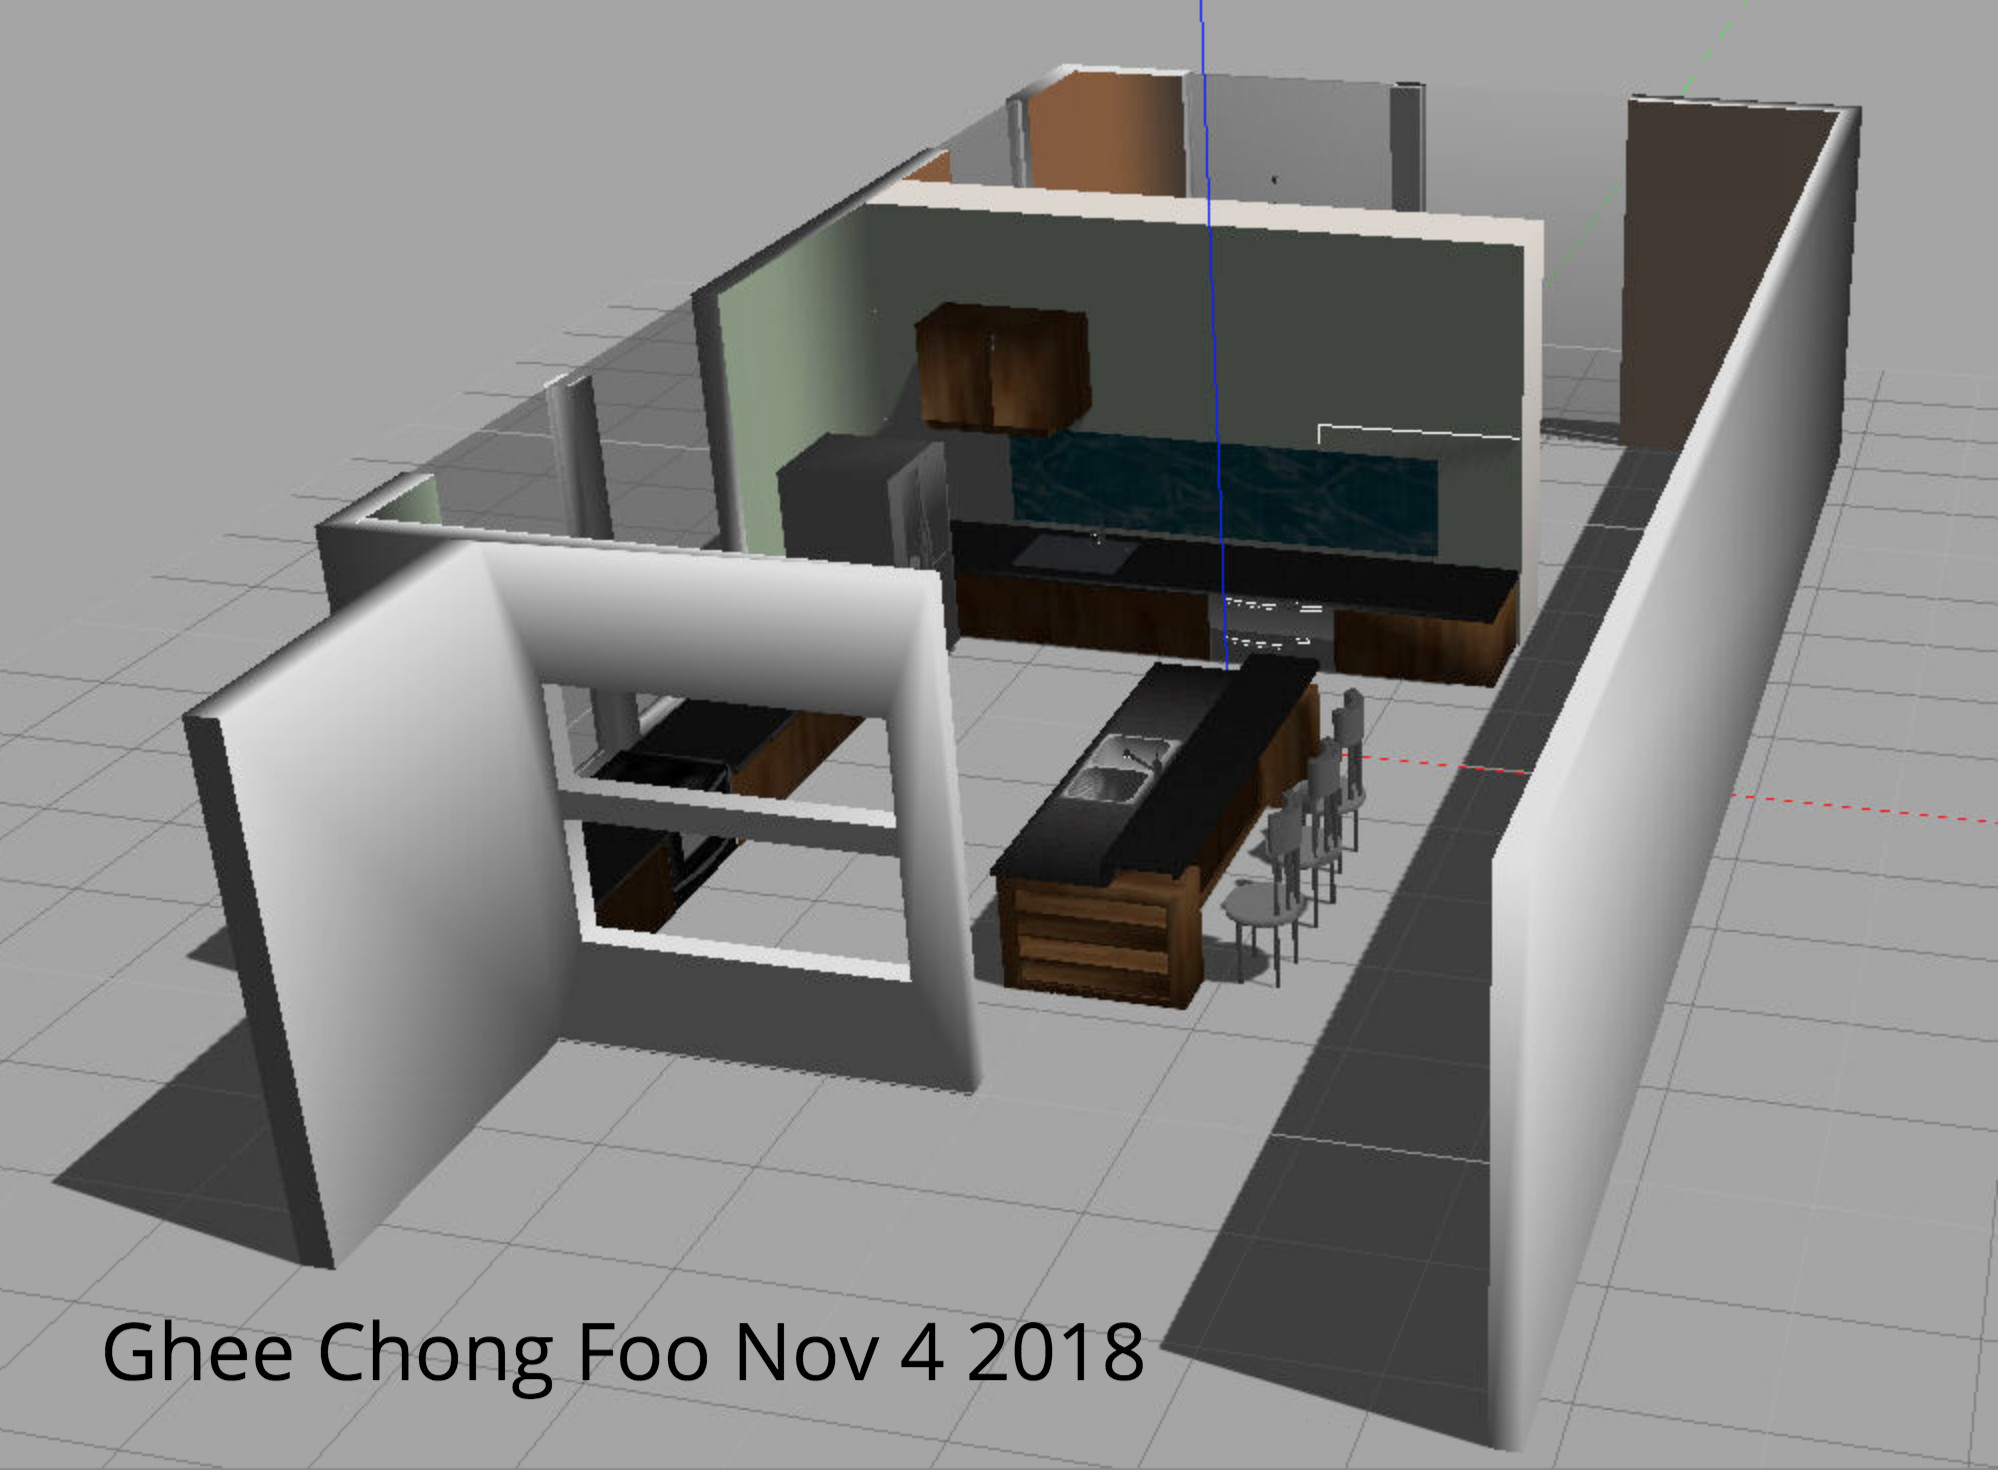
\includegraphics[width=\linewidth]{kitchen_world.png}
      \caption{Kitchen World}
      \label{fig:Kitchen}
\end{figure}

%\subsection{Subsection Heading Here}
%Subsection text here.

%\subsubsection{Subsubsection Heading Here}
%Subsubsection text here.

%example for building table
%\begin{table}[h]
%\caption{Table}
%\label{table_example}
%\begin{center}
%\begin{tabular}{|c||c|}
%\hline
%One & Two\\
%\hline
%Three & Four\\
%\hline
%\end{tabular}
%\end{center}
%\end{table}



\section{Background}

In localization, the problem is estimating the robot's poses given some landmarks, while in mapping the landmarks is estimated given the robot's poses. SLAM take a step further by trying to estimate both the robot's poses and landmarks \textbf{simultaneously}, and hence the name.  Although this has been perceived as chicken-and-egg problem, it is fundamental requirement for robot to be truly autonomous and the basis for most navigation systems.

Two general approach to SLAM problem are Full SLAM and Online SLAM.  In Full SLAM the algorithm tries to estimate the entire path, while Online SLAM seeks to recover only the most recent pose.  The differences between the algorithms is how they differentiate already detected features to keep the map consistent, i.e. solving loop closure problem.

One of the popular SLAM algorithm is FastSLAM, which decomposes the SLAM problem into localization and landmark estimation problem that are conditioned on robot pose estimate. FastSLAM uses a modified particles filter for estimating posterior over robot paths.  By representing maps as a grid, one can get away with the landmarks based approach and estimate a map for any arbitrary environment. It is a combination of robot pose estimation using particle filter and occupancy based mapping algorithm with known poses.

In this project, Graph-SLAM algorithm will be employed.  The algorithm represent the SLAM problem as a graph with poses of the trajectory and measurement locations as nodes as well as using estimated motion and measurement distances as links. The links in the graph are the constraints between the robot poses and its environment represent their relationship. Graph-SLAM then tries to resolve all of these constraints by creating the most likely map on the given data. In particular, the Real Time Appearance Based Mapping (RTAB-Map) is used, which is Graph-SLAM approach that uses bag of words approach to identify correspondences between frames using visual similarity for optimization. The camera image is compared against already known map features allowing the algorithm to map trajectories with repeated locations and thus reducing constraint complexity.

%In robot mapping, the surrounding environment is esti- mated and the path of the robot is assumed to be in the past. A lot of challenges present themselves while mapping like
%• infinite variables to describe a map as a continous space
%• uncertainty in perception
%• feature-richness of the space to be mapped
%SLAM takes this challenge a step further: additionally to constructing a map of the environment, the robot simultane- ously localizes itself relative to its map. Its a basic feature for autonomous mobile robots. Neither the map nor the robot poses are provided and both will inhabit noise from the sensors measurements. This could lead to an uncertain map and errors in the pose estimates. The problem is approached in two variations: Online SLAM estimates current pose and map from previous measurements and motions, Full SLAM estimates the entire trajectory and map features at the same time.
%A SLAM algorithm has to identify correspondences be- tween images to correctly resolve map features. Basic SLAM works like this: The robot starts with measurement zero on its initial pose and includes it into the map. Then the robot moves and takes another measurement, calculates its new
%position from the current map and includes the new unseen features into the map. This way, the map is incremented continually. The differences between the algorithms is how they detect already seen features to keep the map consistent - this is called the loop closing problem.

%The SLAM method used in this experiment is a Graph- SLAM algorithm. These types of algorithms represent the SLAM problem as a graph with poses of the trajectory and measurement locations as nodes as well as estimated motion and measurement distances as links. The links in the graph are the contraints between the robot poses and its environment and represent their relationship. GraphSLAM tries to resolve all of these constraints to create the most likely map on the given data. In this project, the algorithm Real Time Appearance Based Mapping (RTAB-Map) is used. It is an upgraded version of GraphSLAM which uses a bag of words approach to identify correspondences between frames using visual similarity. Every frame, the camera image is compared against already known map features allowing to map trajectories with repeated locations by reducing constraint complexity.

%Background - The student provides a sufficient background into the scope of the problem / technologically while also identifying some of the current challenges in robot mapping and why the problem domain is an important piece of robotics. They further discuss and compare mapping algorithms


\section{Scene and robot configuration}
%Student explains how the gazebo world was created by providing an overview of the layout of items in his/her customized Gazebo world. Student also describes the robot's parameters, sensor features, and reasoning on the package structure. 

The initial environment can be reproduced by running "create\_workspace.bash" script in Github depo, which consists of following commands:

\begin{verbatim}
#!/bin/bash

mkdir -p ~/catkin_ws/src
cd ~/catkin_ws/src
catkin_init_workspace
cd ~/catkin_ws
catkin_make; source devel/setup.bash
cd ~/catkin_ws/src
git clone 
https://github.com/ggnohc/RoboND-MapMyWorld.git
cd ~/catkin_ws
catkin_make; source devel/setup.bash
\end{verbatim}

The udacity provided kitchen dining world and custom world, and the relevant services can be launch through following:
\begin{itemize}
\item roslaunch udacity\_bot udacity\_world.launch
\item (or) roslaunch udacity\_bot Office.launch
\item roslaunch udacity\_bot teleop.launch
\item roslaunch udacity\_bot mapping.launch
\item roslaunch udacity\_bot rviz.launch
\end {itemize}

5 launch file has been created/provided as below:
\begin{enumerate}
    \item \textbf{udacity\_world.launch}: Launches the kitchen dining world and the robot model
    \item \textbf{Office.launch}: Launches the custom model (to be elaborated later)
    \item \textbf{teleop.launch}: Launches the teleop movement to control robot movement manually
    \item \textbf{mapping.launch}: Launches RTAB-map services to providing mapping and closure
    \item \textbf{rviz.launch}: Launches RViz for robot\_slam.rviz configuration
\end{enumerate}

\subsection{Scene configuration}
\begin{figure}[thpb]
      \centering
      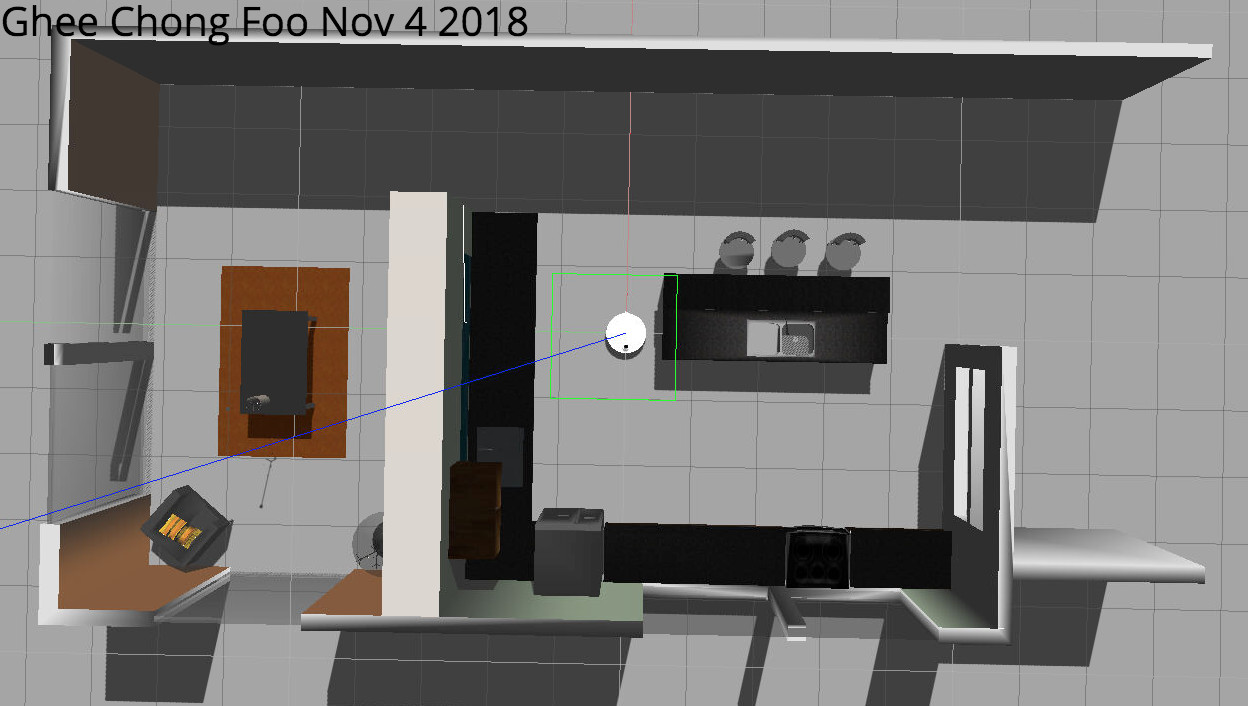
\includegraphics[width=\linewidth]{kitchen_world_top_view.png}
      \caption{Kitchen World}
      \label{fig:kitchen_top}
\end{figure}

Figure ~\ref{fig:kitchen_top} depicts top view of Kitchen Dining World as part of student material.

\begin{figure}[thpb]
      \centering
      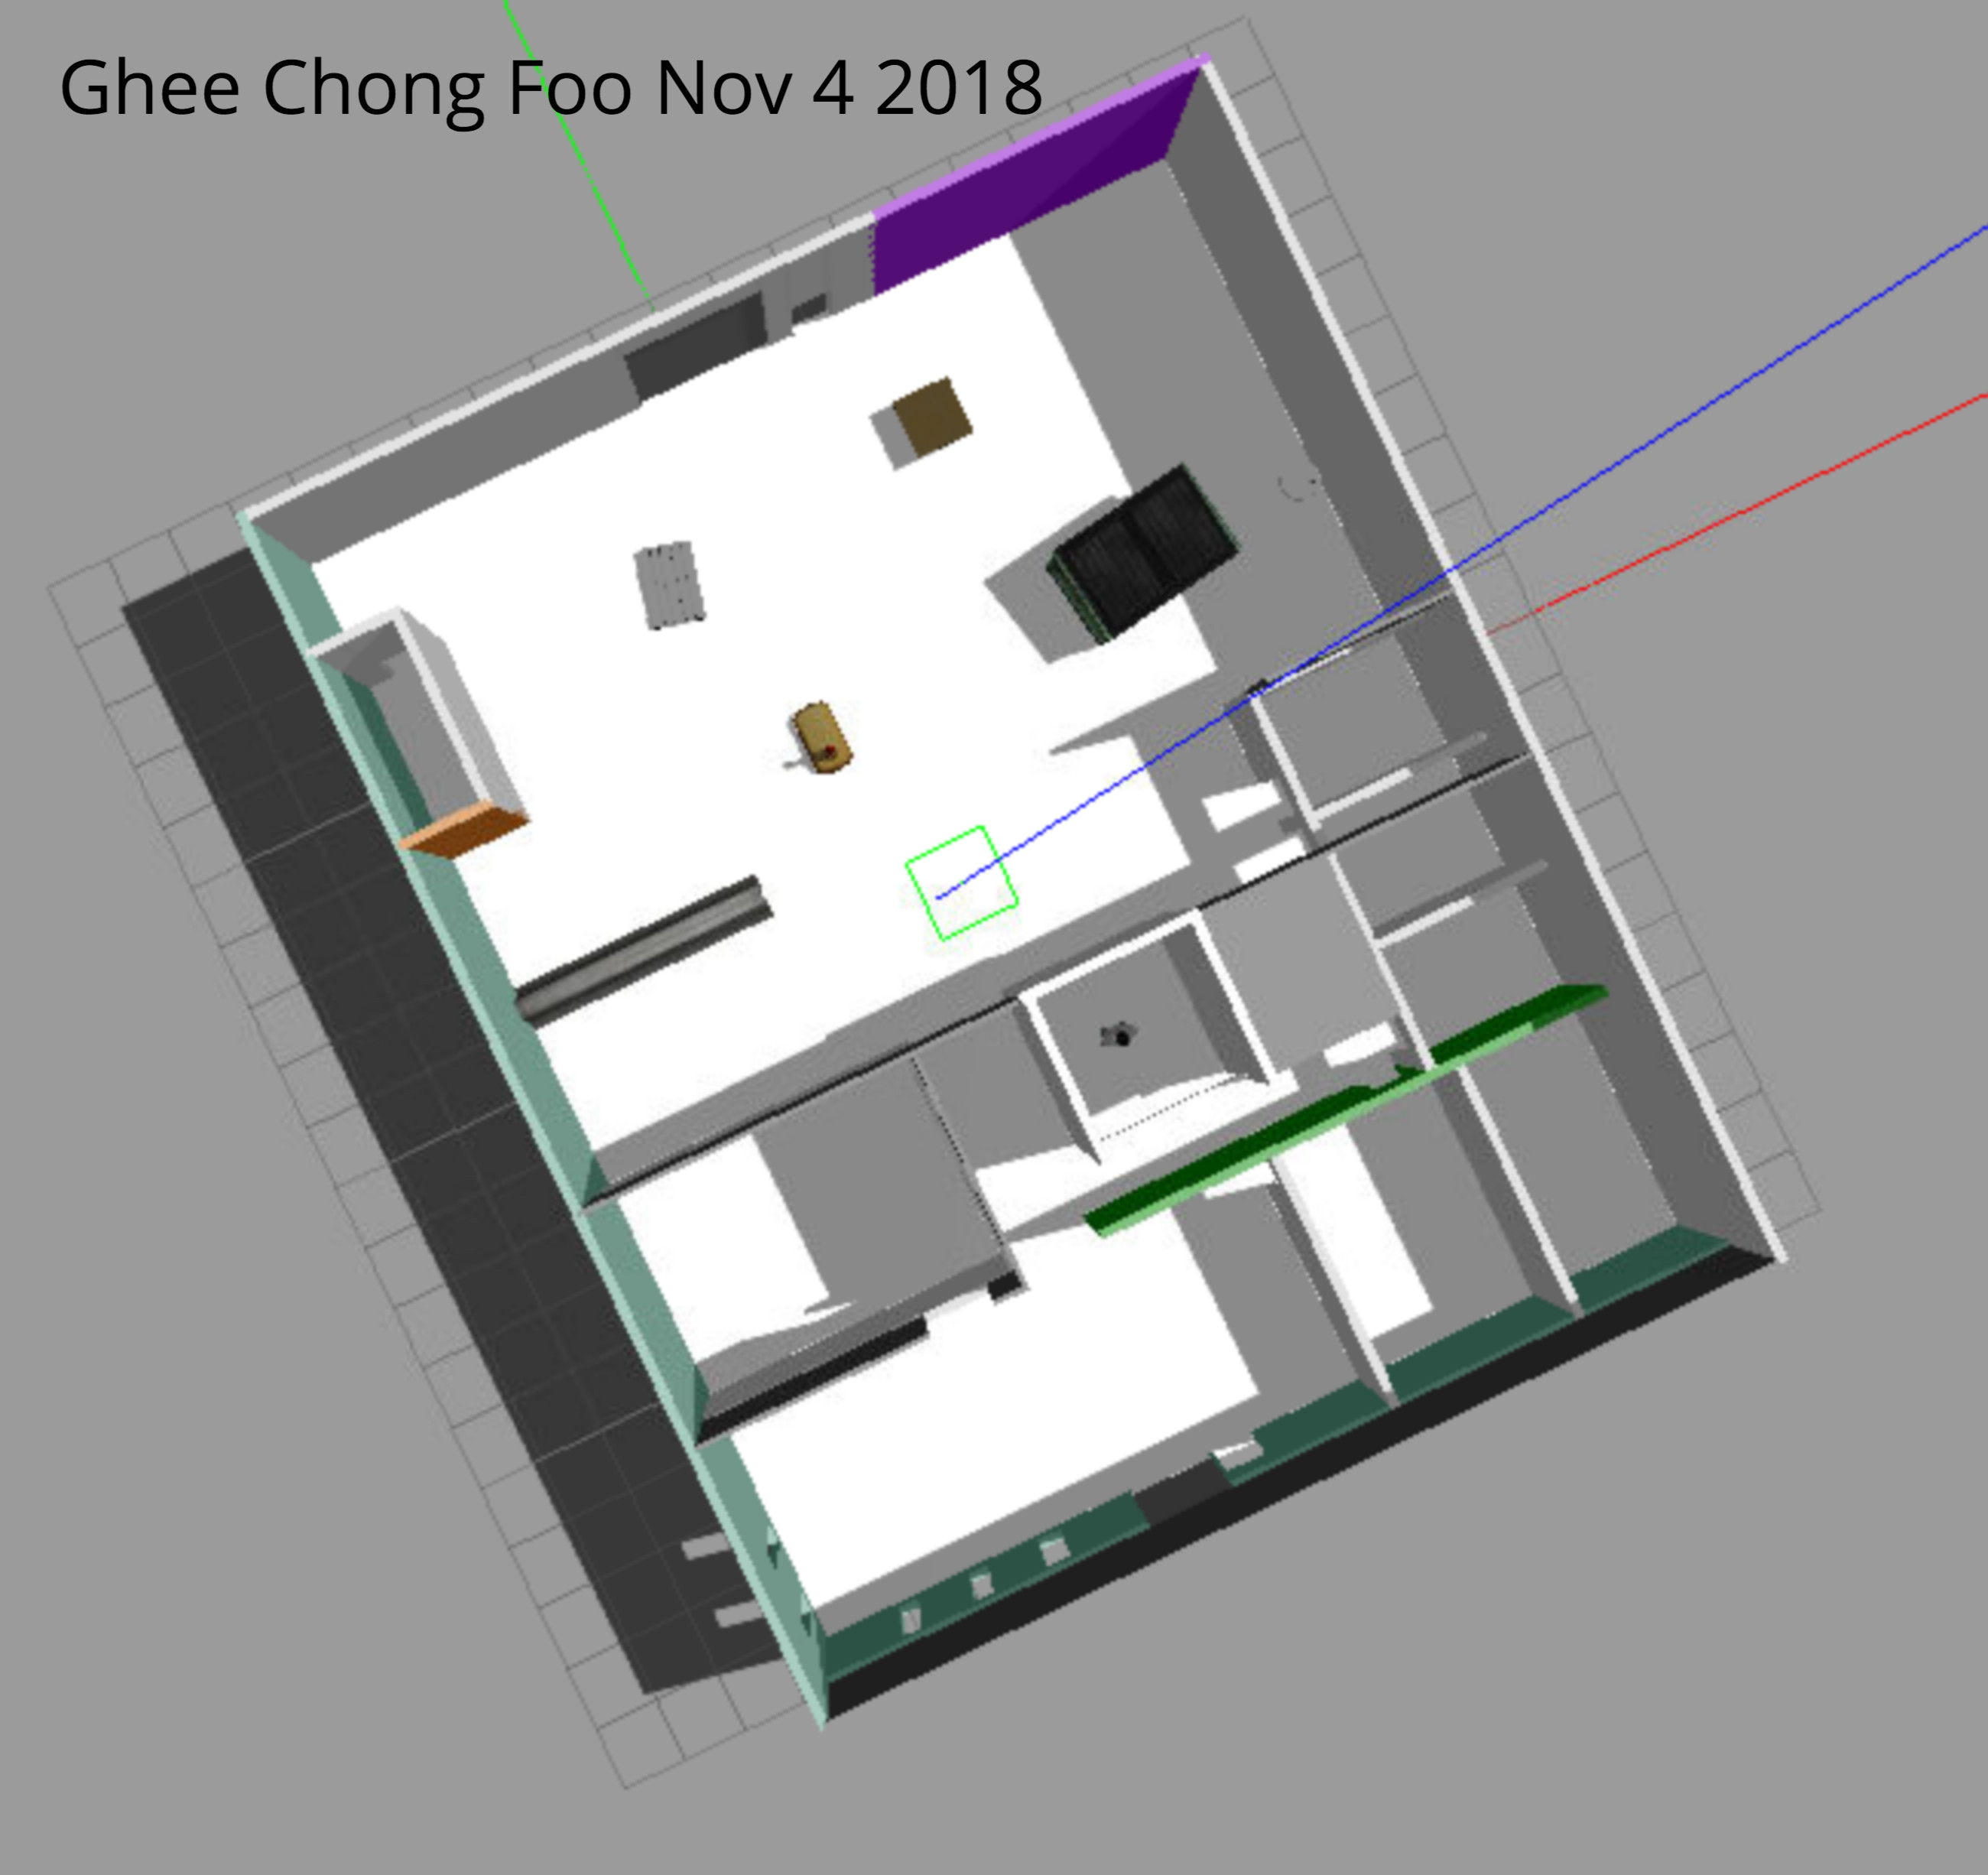
\includegraphics[width=\linewidth]{Office_World.png}
      \caption{Office World}
      \label{fig:office_top}
\end{figure}

Figure ~\ref{fig:office_top} depicts custom created Gazebo world, which is based on Gazebo OSRF Elevator model, and populated with miscellaneous items such as standing person, cafe table, dumpster etc. for mapping purpose.

\subsection{Robot configuration}
\begin{figure}[thpb]
      \centering
      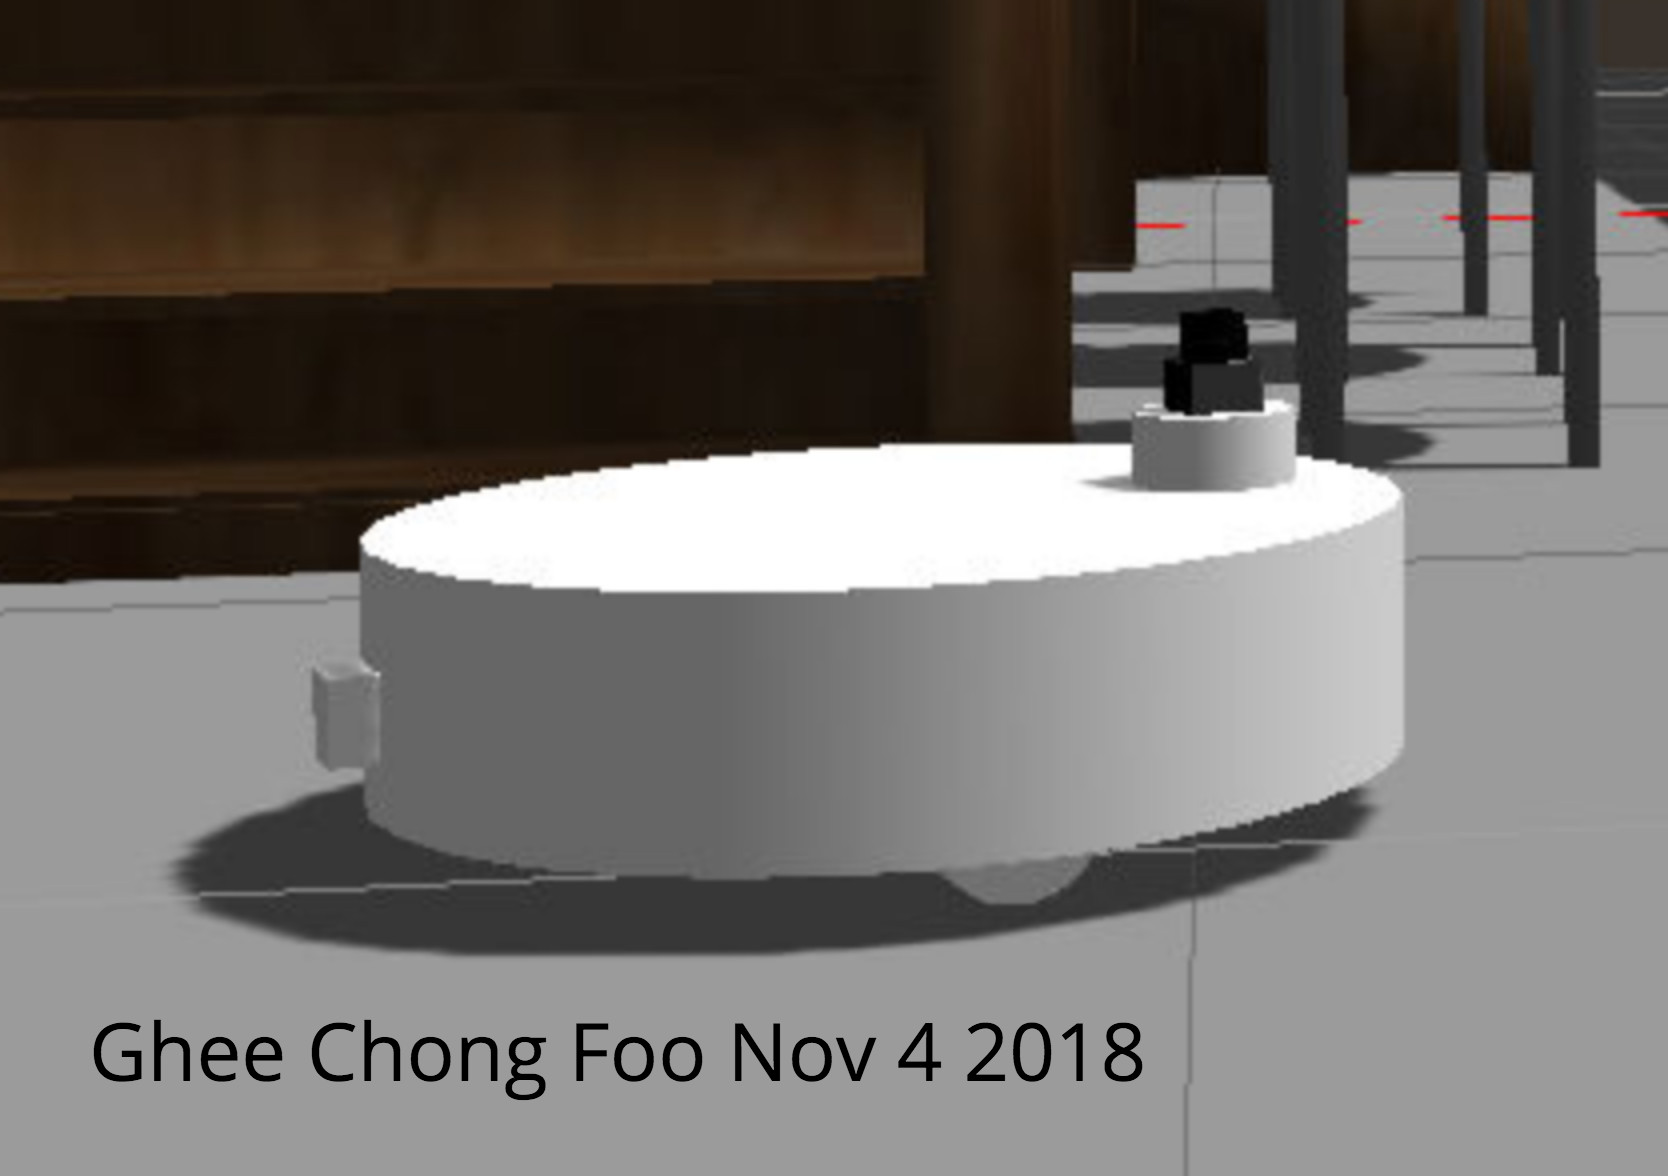
\includegraphics[width=\linewidth]{robot_model.png}
      \caption{Robot Model}
      \label{fig:robot_model}
\end{figure}

The robot is modelled after house hold vacuum cleaning robot, having a cylinder shape and depth camera mounted at the top and camera mounted at the front, as in Figure ~\ref{fig:robot_model}.  

\begin{figure}[thpb]
      \centering
      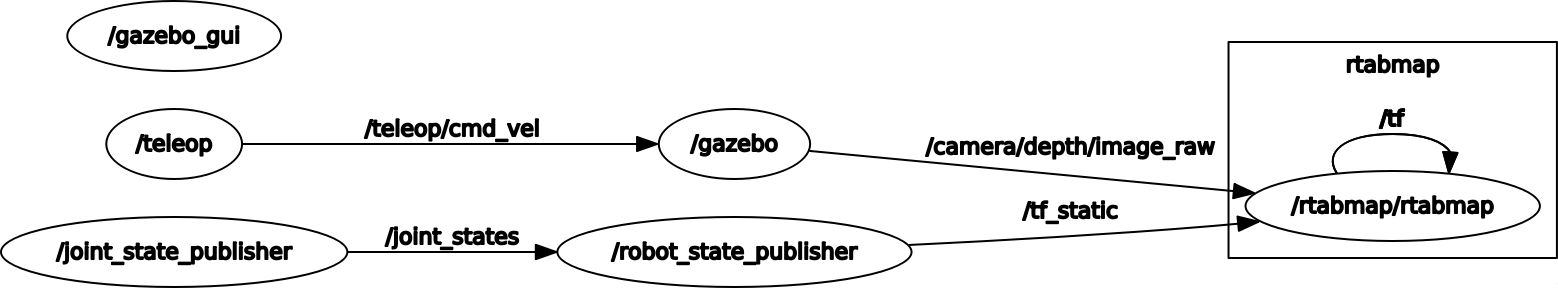
\includegraphics[width=\linewidth]{rosgraph.png}
      \caption{rosgraph for robot model}
      \label{fig:rosgraph}
\end{figure}

Figure ~\ref{fig:rosgraph} shows the ROS Graph for the robot model.

\section{Results}
%The student should include the images for mapping process, final map (2D/3D) for both Gazebo worlds.
The robot was driven manually through teleop control, often passing through the same area multiple times to make sure the area was detected by observing the point cloud in Rviz.  In both world the minimum required of 3 loop closure was achieved.

The RTAB-MAP database is archived in \url{https://drive.google.com/open?id=1Orfo77AVvk9UFrvDMlLDa_U68EGVkIPb}

\subsection{Kitchen Dining World}

\begin{figure}[thpb]
      \centering
      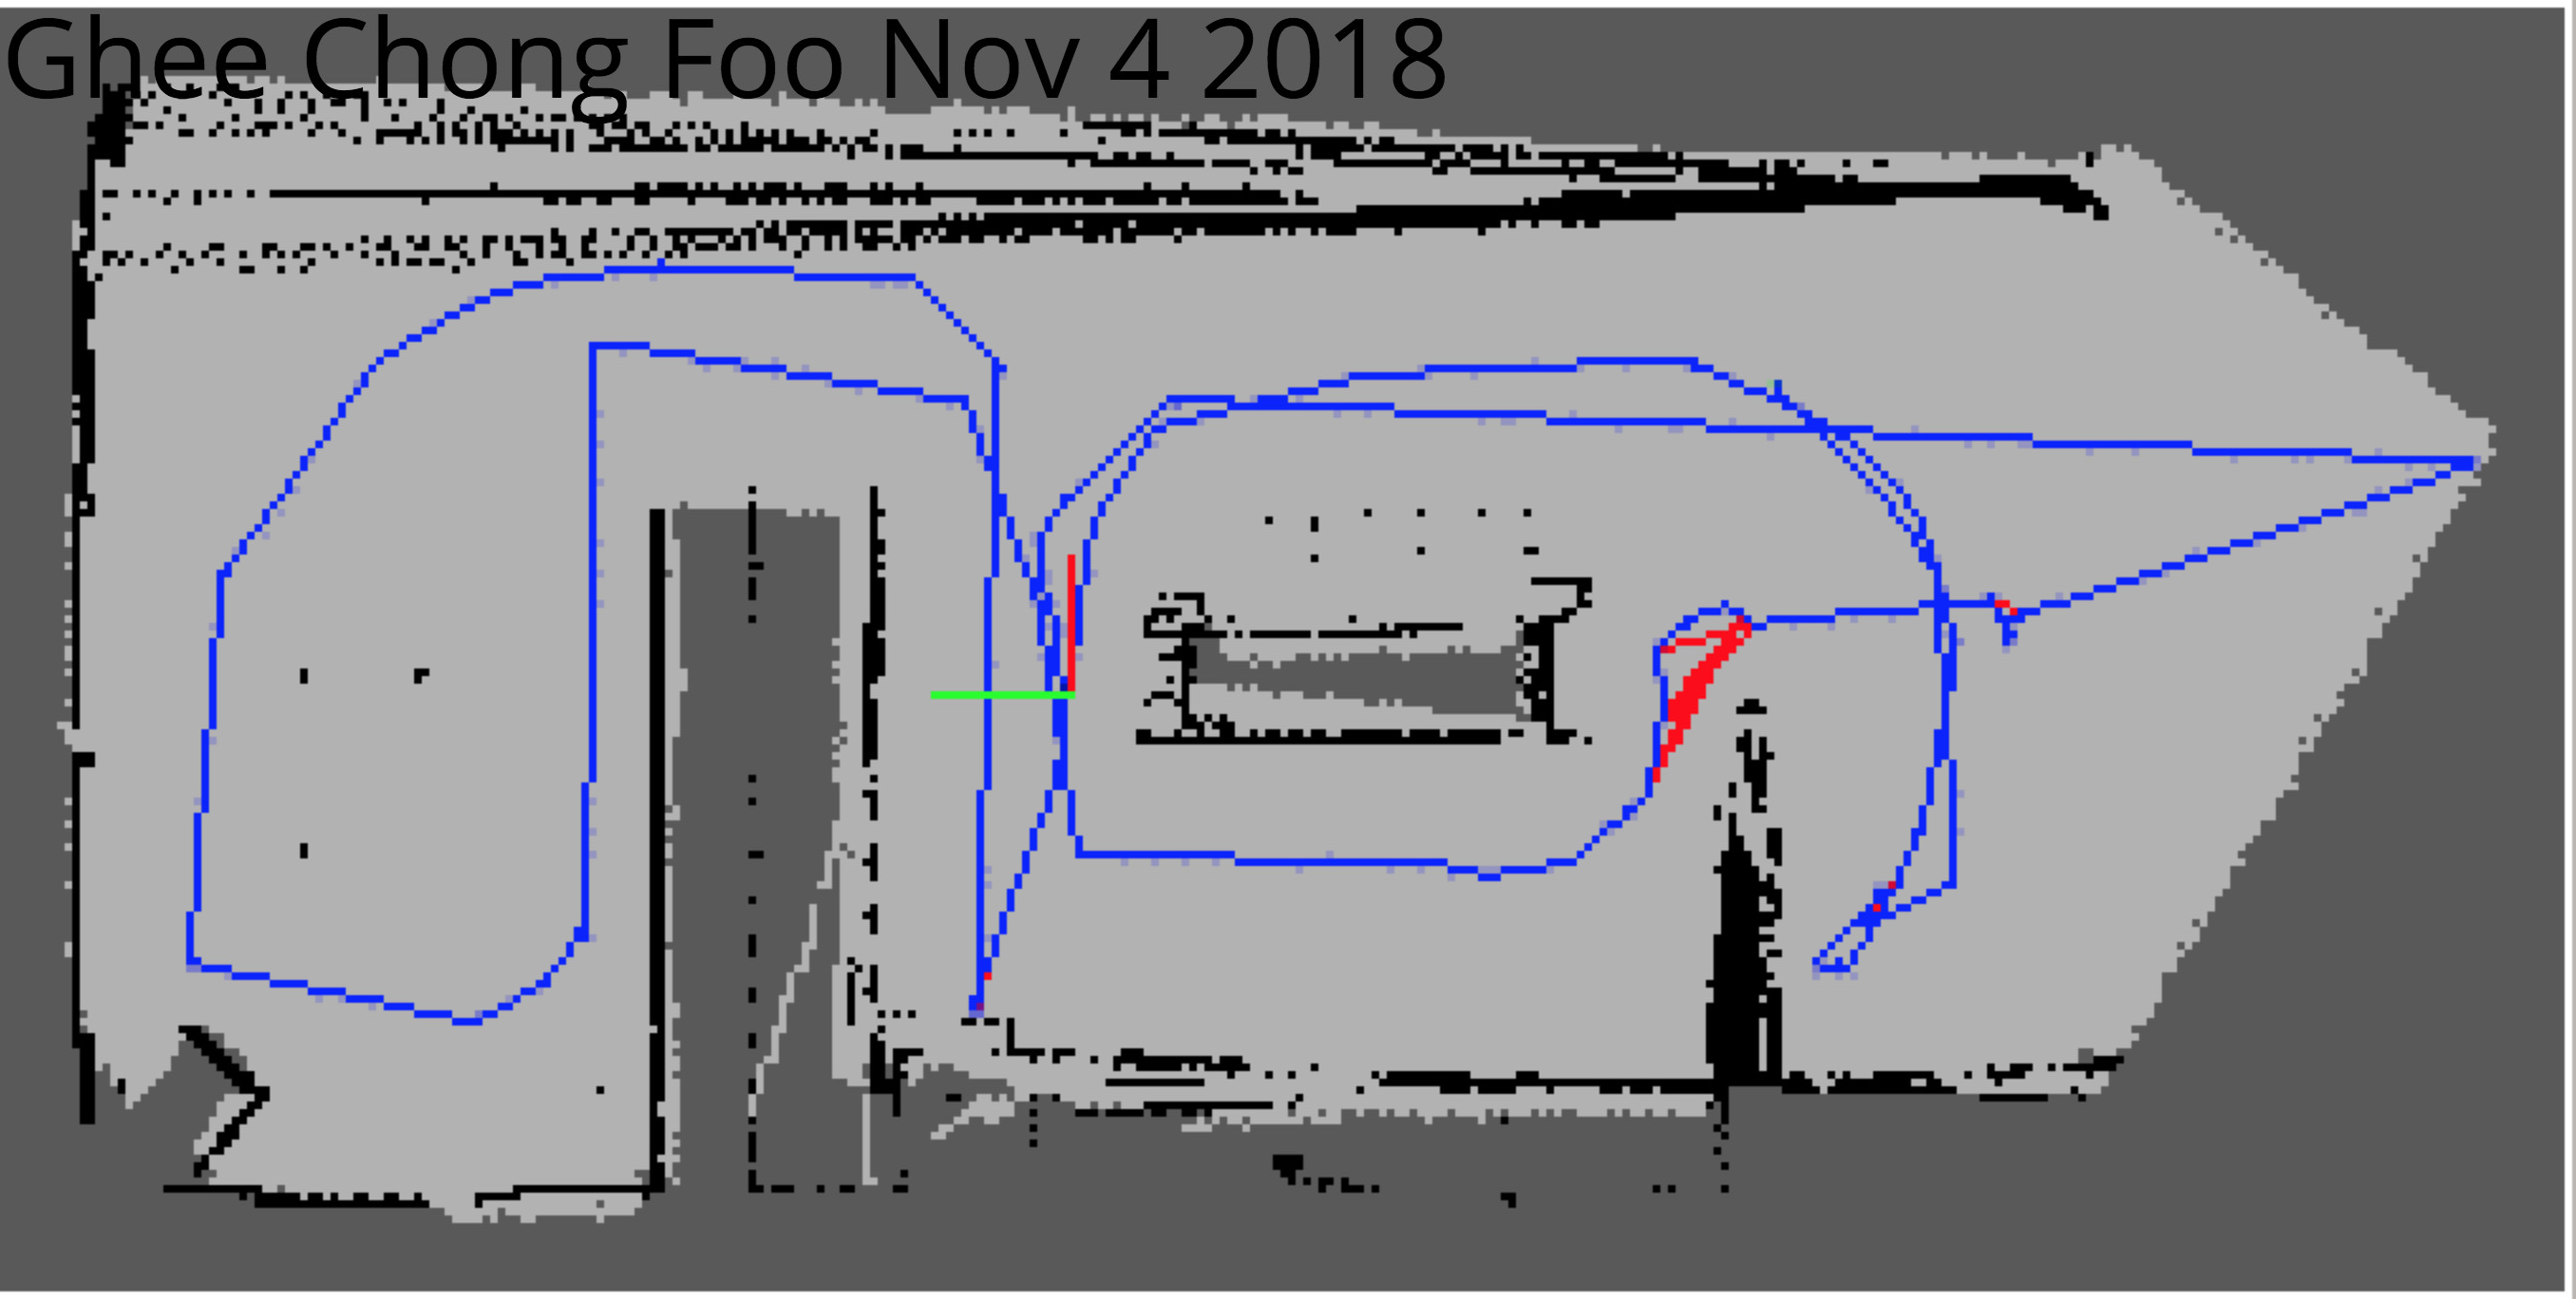
\includegraphics[width=\linewidth]{Kitchen_2D.png}
      \caption{Kitchen 2D}
      \label{fig:kitchen_2d}
\end{figure}

Figure ~\ref{fig:kitchen_2d} shows the path that robot has pass through while mapping the Kitchen world.

\begin{figure}[thpb]
      \centering
      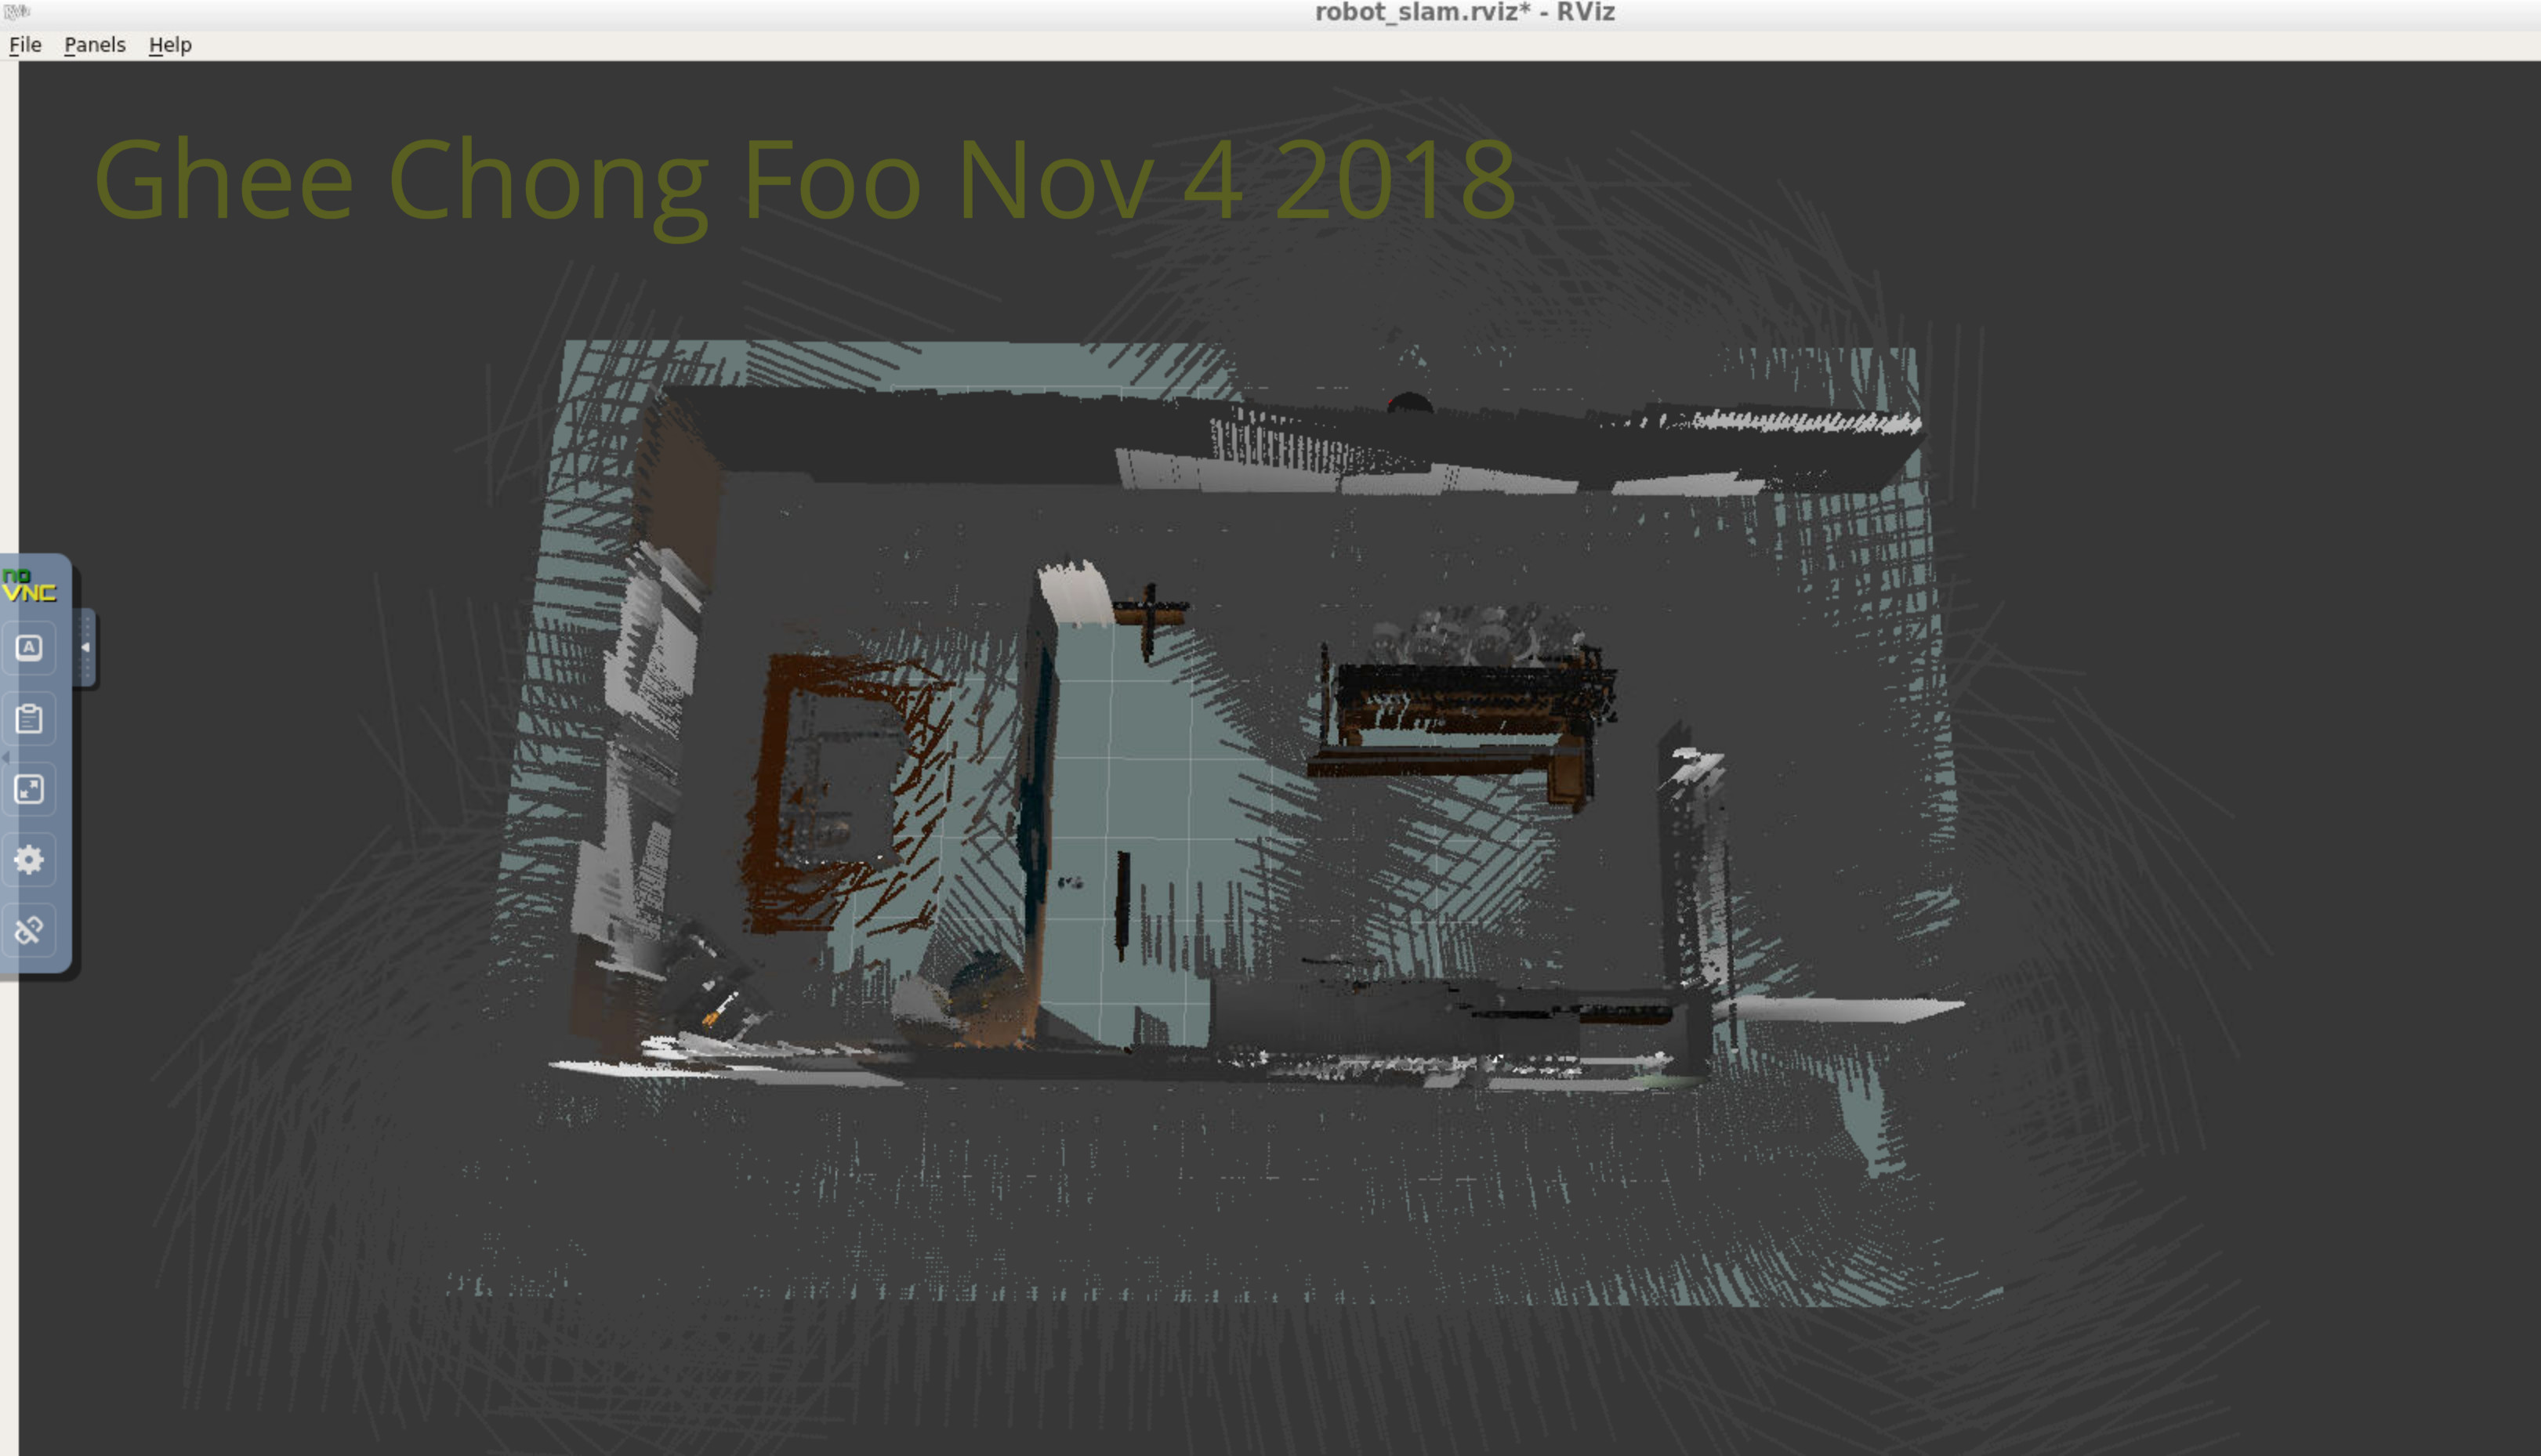
\includegraphics[width=\linewidth]{Kitchen_World_3D.png}
      \caption{Kitchen 3D}
      \label{fig:kitchen_3d}
\end{figure}

Figure ~\ref{fig:kitchen_3d} shows the surrounding mapped by the robot presented in 3D.

\begin{figure}[thpb]
      \centering
      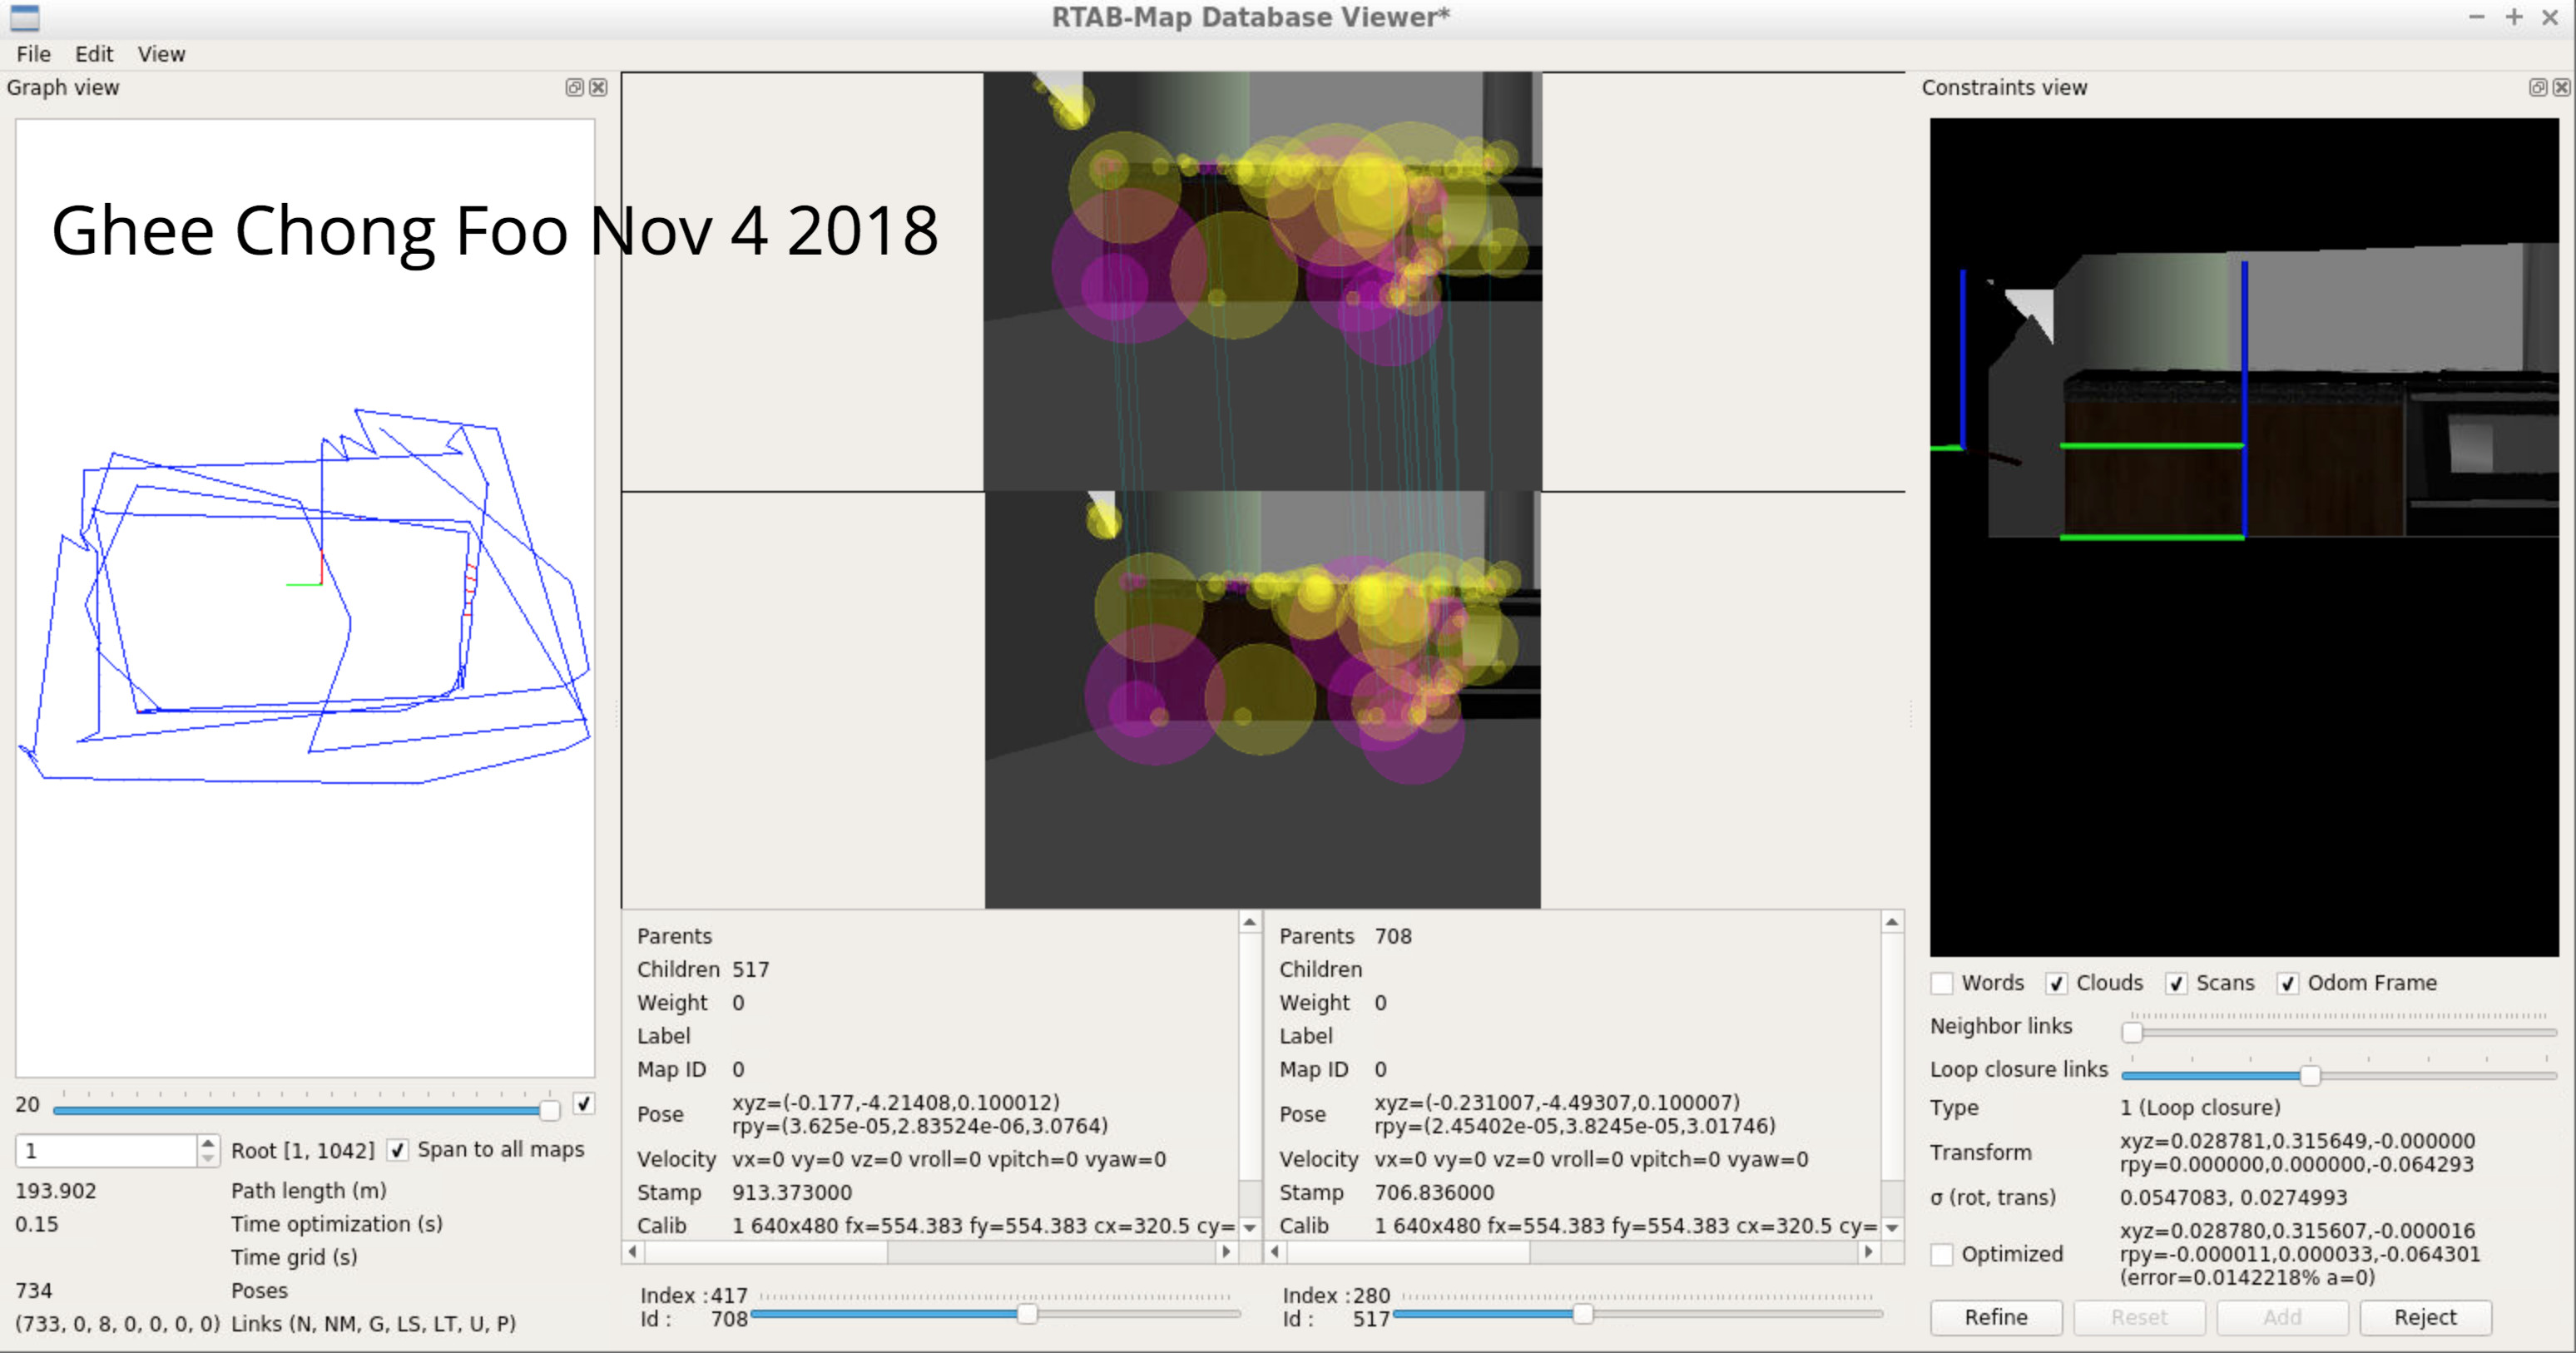
\includegraphics[width=\linewidth]{Kitchen_World_RTAB_Map.png}
      \caption{Kitchen RTAB Map}
      \label{fig:kitchen_rtabmap}
\end{figure}

Figure ~\ref{fig:kitchen_rtabmap} shows the output of RTAB Map database viewer.  8 loop closure has been achieved in this case.

\subsection{Custom Model}


\begin{figure}[thpb]
      \centering
      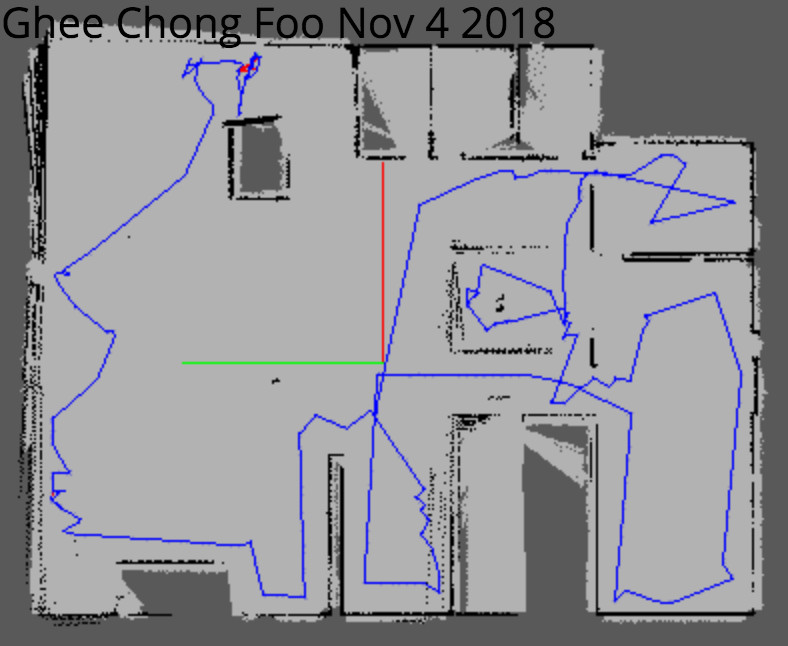
\includegraphics[width=\linewidth]{Office_2D.png}
      \caption{Office 2D}
      \label{fig:office_2d}
\end{figure}

Figure ~\ref{fig:office_2d} shows the path that robot has pass through in Office world.

\begin{figure}[thpb]
      \centering
      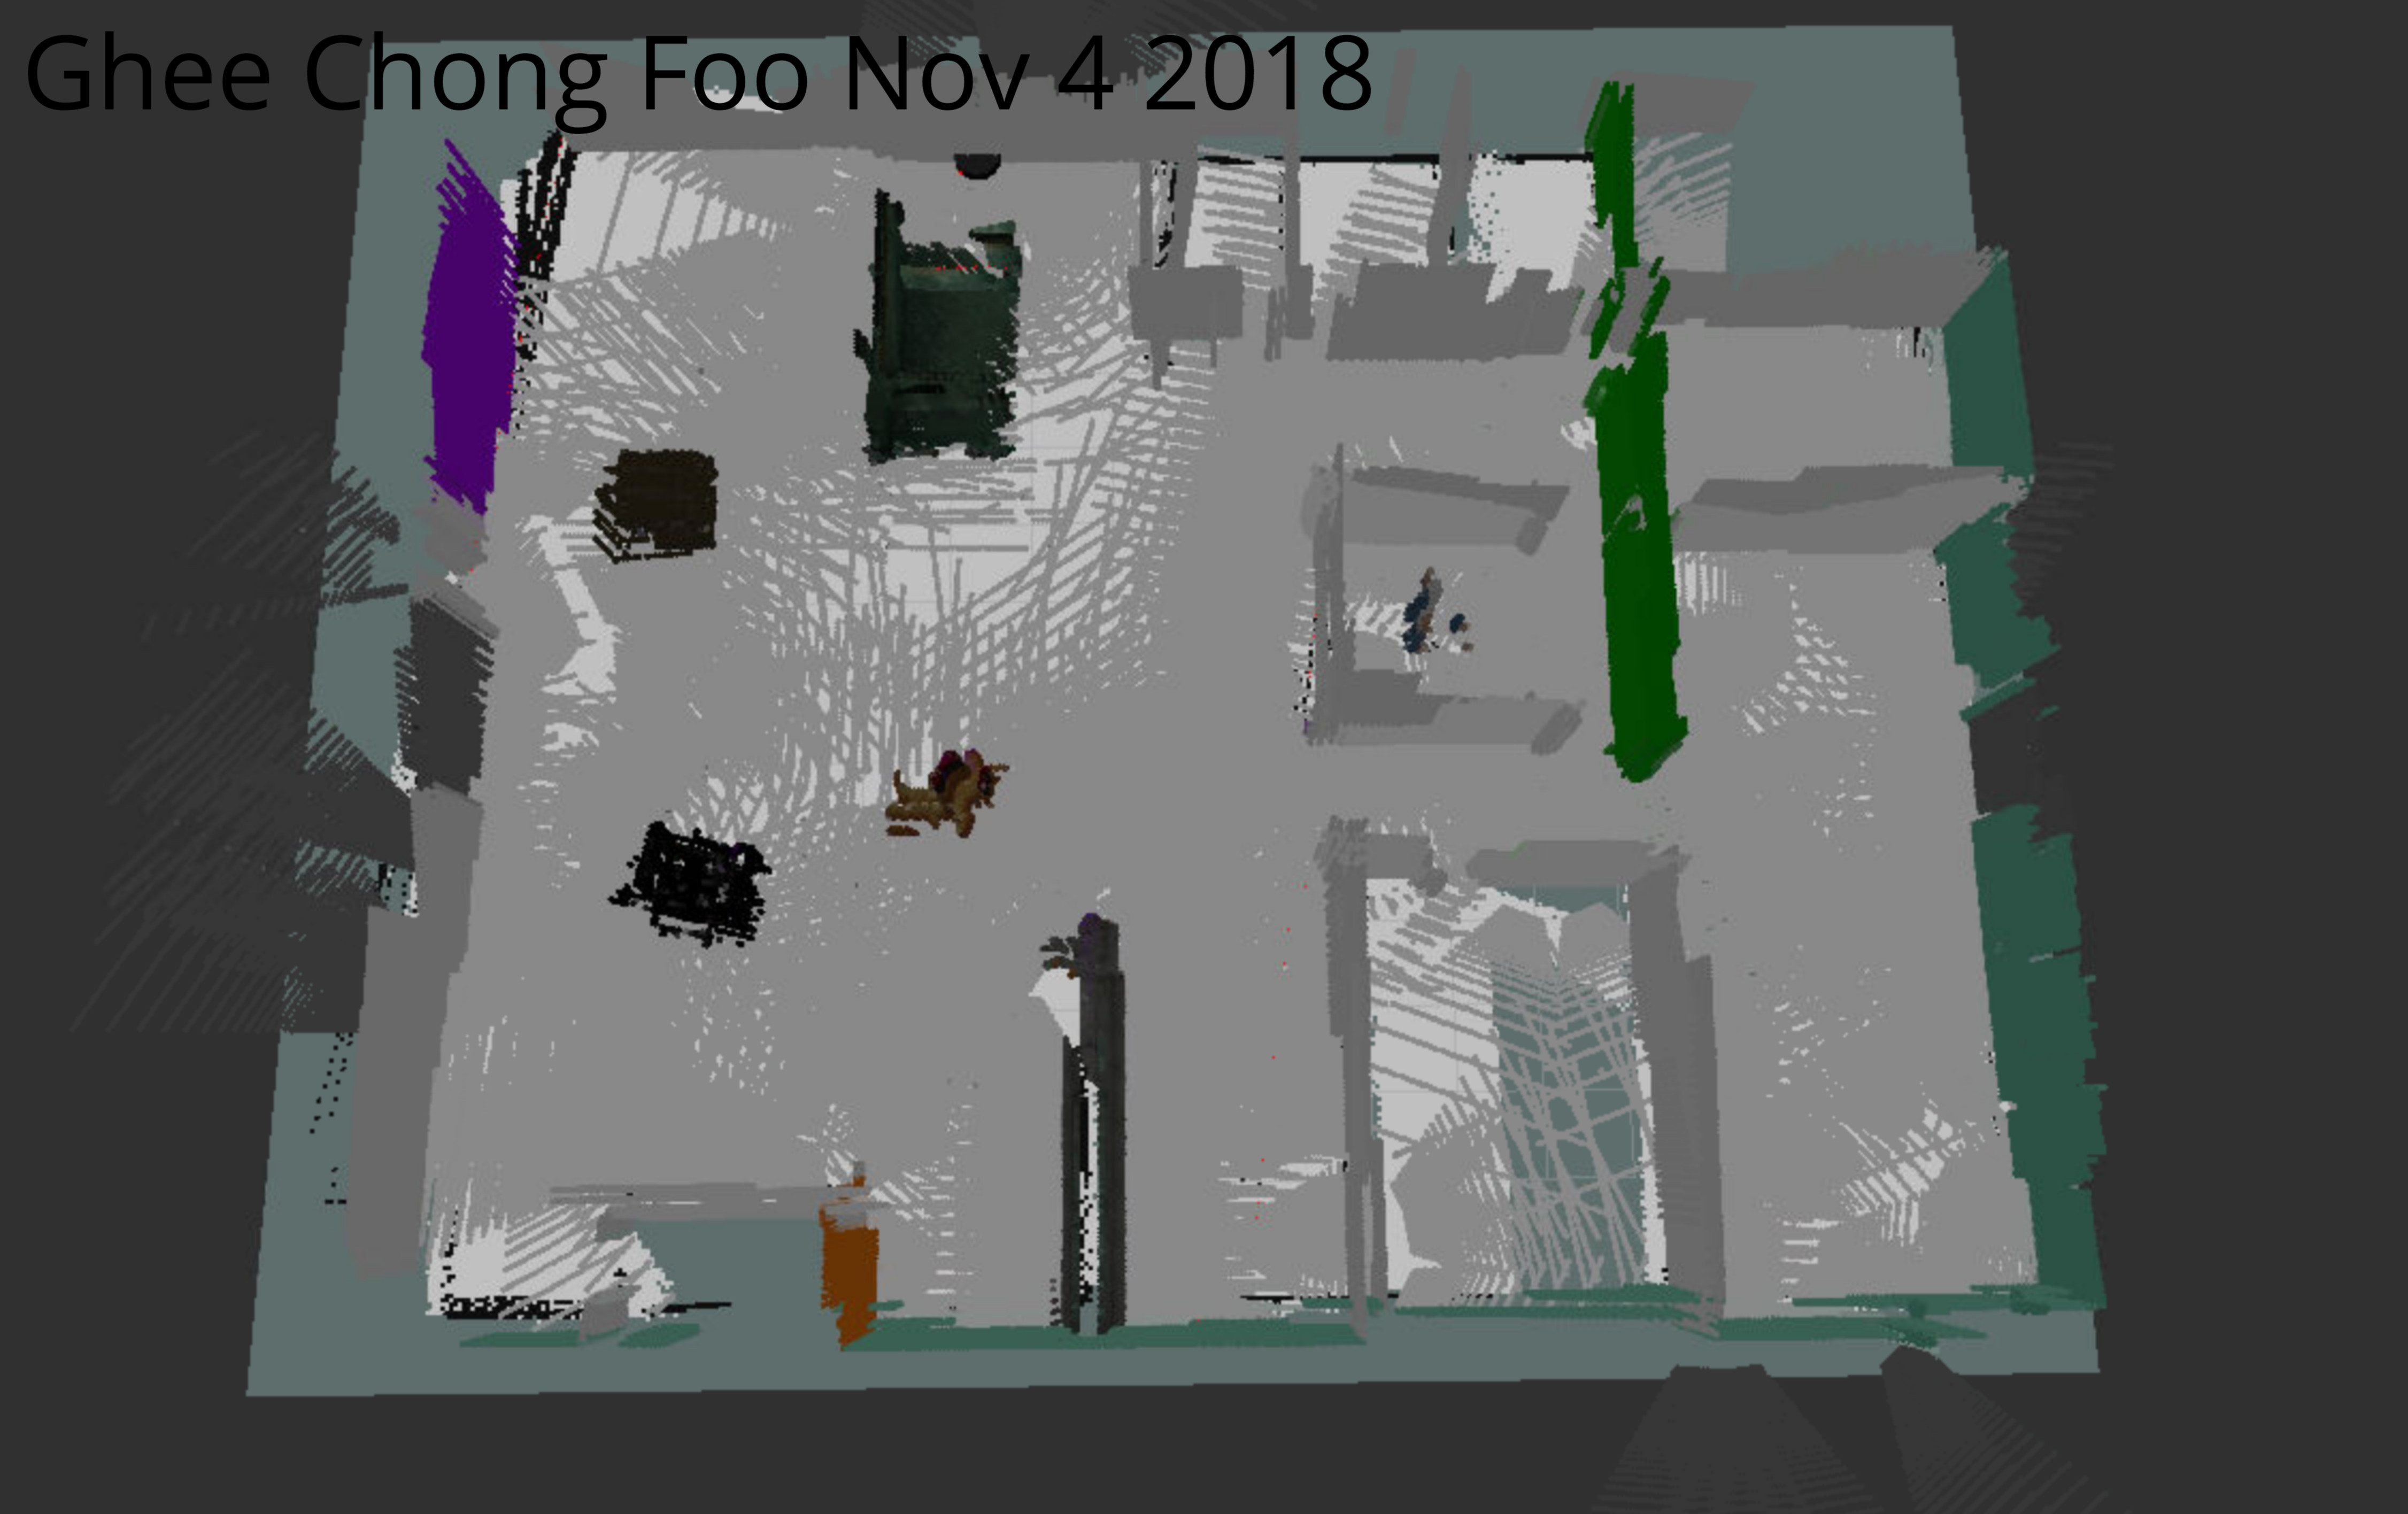
\includegraphics[width=\linewidth]{Office_3D.png}
      \caption{Office 3D}
      \label{fig:office_3d}
\end{figure}

Figure ~\ref{fig:office_3d} shows the Office world mapped by the robot presented in 3D.

\begin{figure}[thpb]
      \centering
      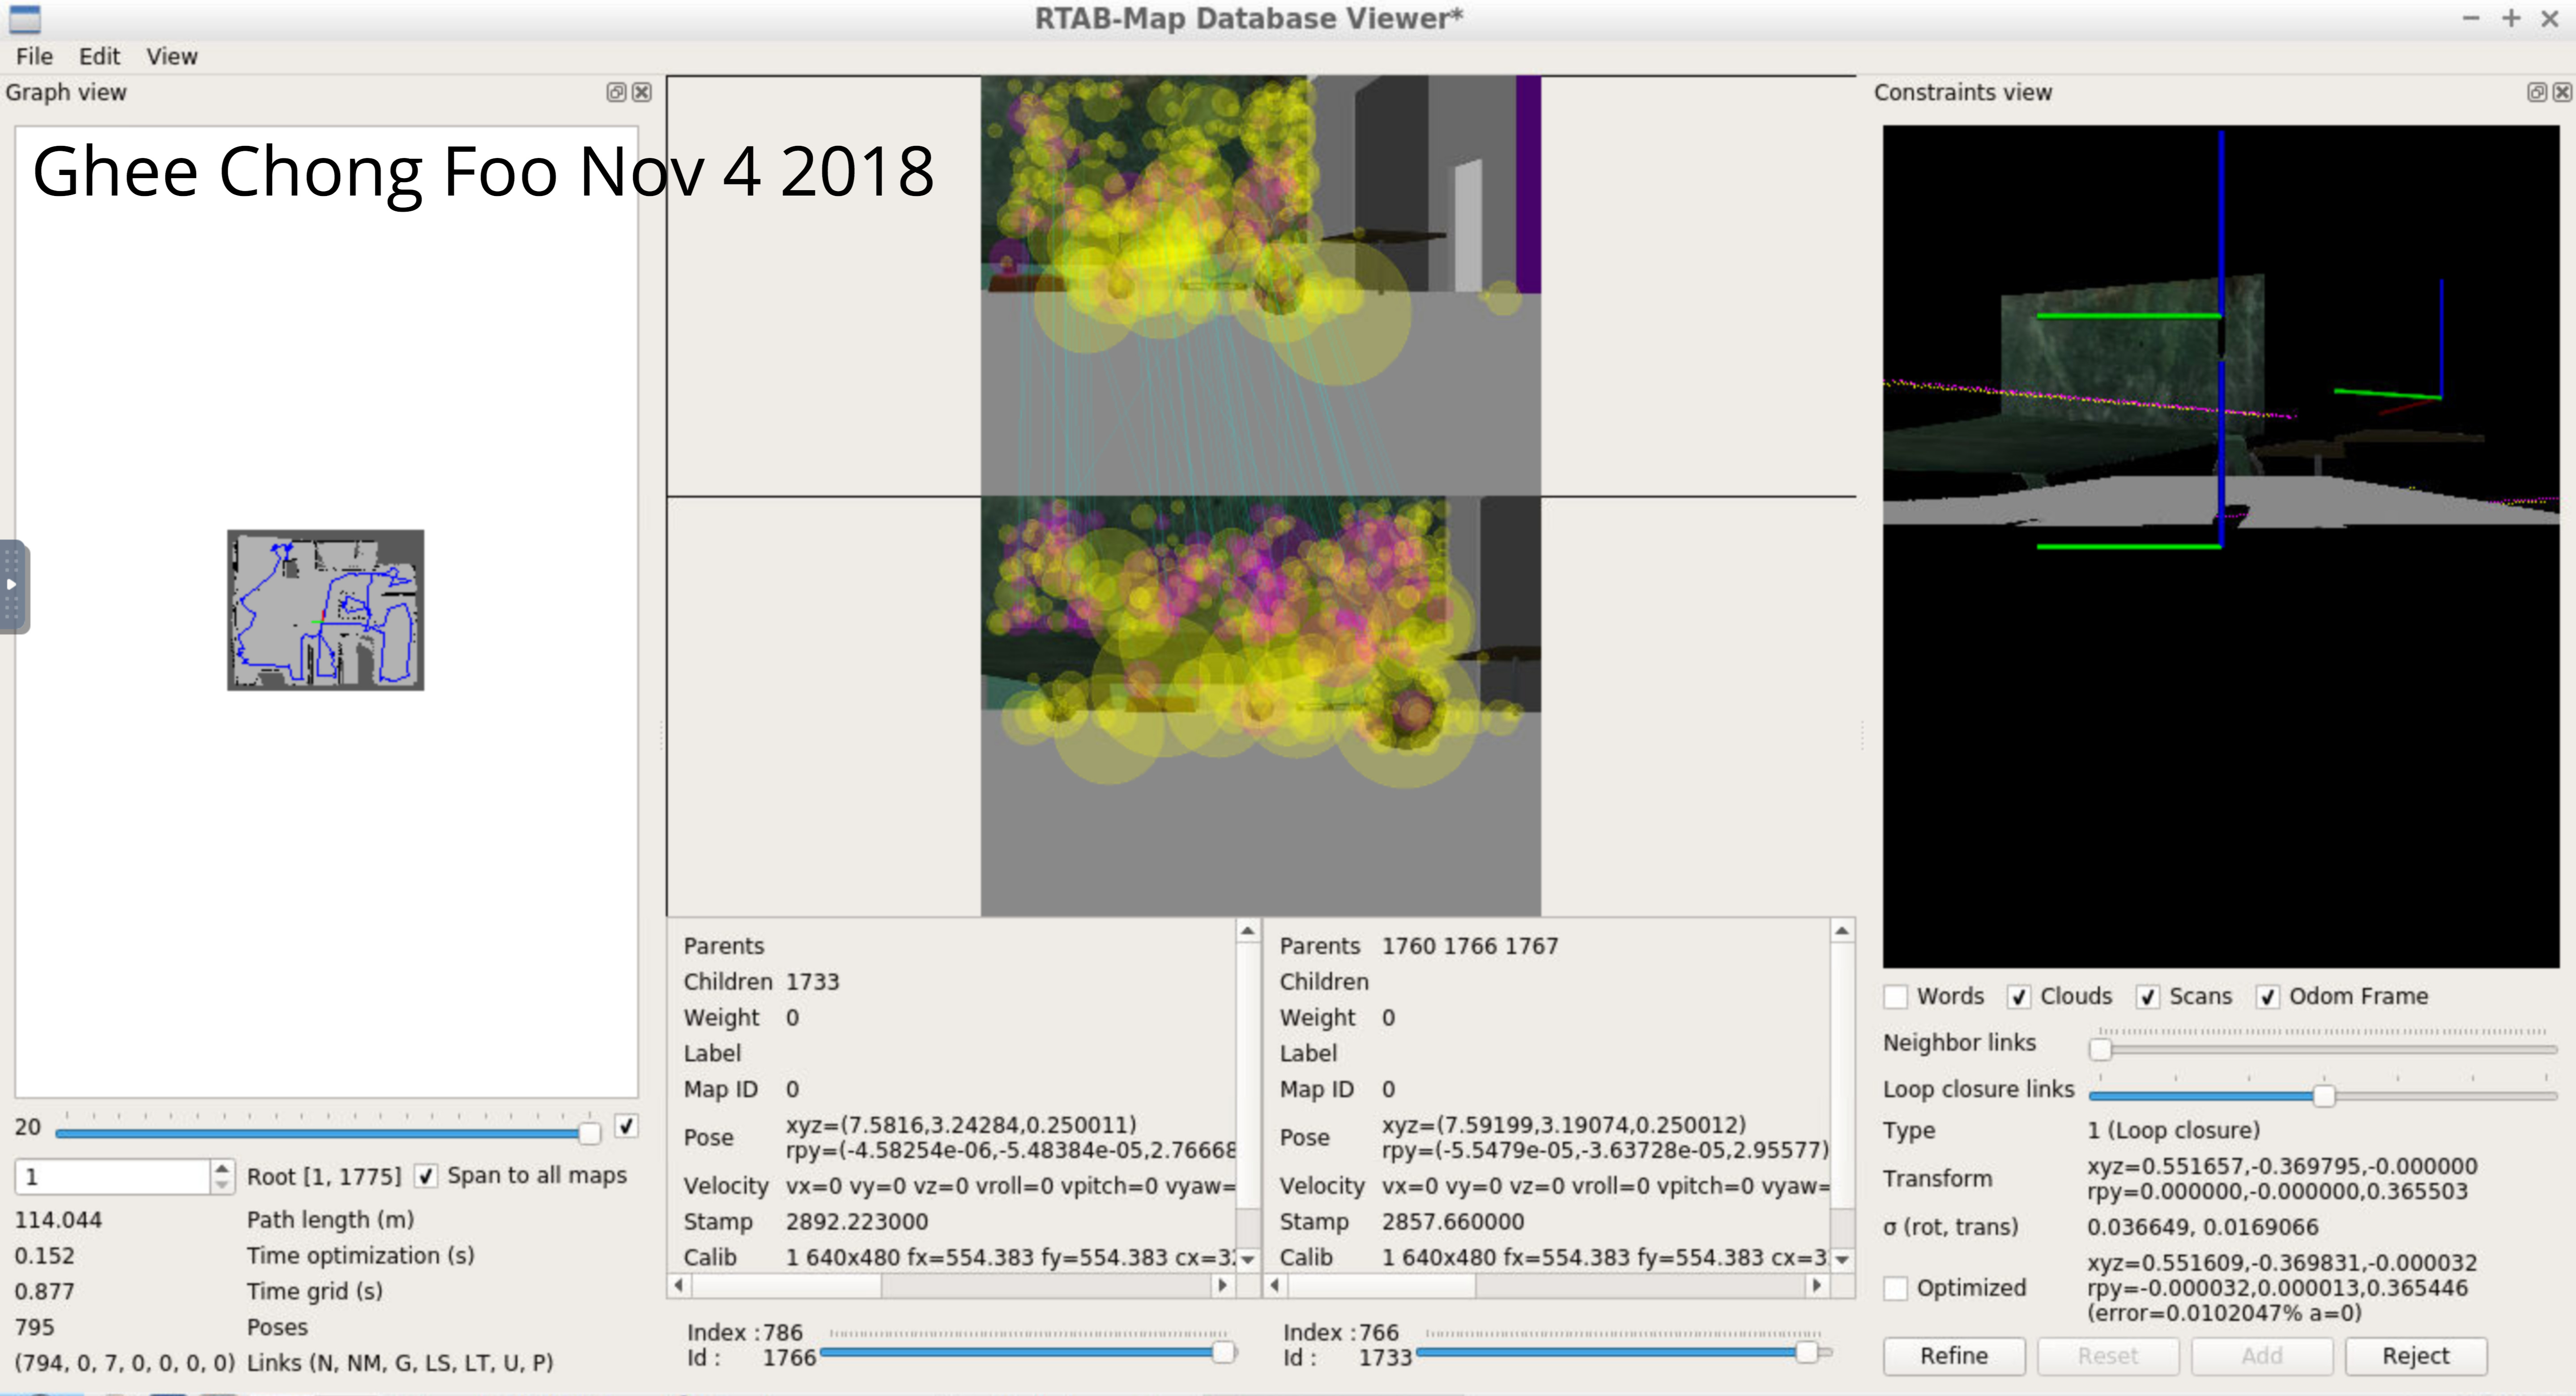
\includegraphics[width=\linewidth]{Office_RTAB_Map.png}
      \caption{Office RTAB Map}
      \label{fig:office_rtabmap}
\end{figure}

Figure ~\ref{fig:office_rtabmap} shows the output of RTAB Map database viewer.  7 loop closure has been achieved in this case.

\section{Discussion}
%The student explains how the procedure went and methodologies to improve it. The student should compare and contrast the performance of RTAB Mapping in different worlds.
 
The Kitchen world was easier to map as it contain object with different sizes and shapes, which is feature rich enough for the RTAB-Map algorithm to identify the environment.  In contrast for the custom office environment, initially it was hard for the robot to map out the environment as it was repetitive and feature-less, which confuses the algorithm and not able to recreate the actual environment.  Once more unique objects are placed then only the robot was able to perform the mapping correctly.  

The map for both world can be further improved by going through the environment several times, by covering angles that was previously missed.  However one will quickly discover that the size of the RTAB-Map database grows quickly and might not scale in a large and complex environment.

\section{Future work}
%The student can discuss how they would like to leverage this tool in robotics. The student identifies other areas where mapping could be done and for what reason. Such as simulated room or physical place. 

RTAB-Map is an interesting application of GraphSLAM algorithm.  Future work would include running it in a actual mobile robot instead of simulation, which has to deal with real world noise such as those coming from camera and actuator due to imperfect sensor and environment.  While RTAB-Map works well in mapping static and feature rich environment, more works are needed to deploy the robot in a dynamic environment, such as busy hospitals with people constantly moving around versus static walls or rooms.








\bibliography{bib}
\bibliographystyle{ieeetr}

\end{document}